\documentclass[11pt]{beamer}
\usepackage[utf8]{inputenc}
\usepackage[T1]{fontenc}
\usepackage[french]{babel}
\usepackage{graphicx}
\usepackage{tikz}
\usepackage{pgfgantt}
\usepackage{hyperref}
\usepackage{xcolor}
\usepackage{listings}

\usetheme{Madrid}
\usecolortheme{default}

% Configuration pour le code
\lstset{
    basicstyle=\tiny\ttfamily,
    keywordstyle=\color{blue},
    commentstyle=\color{gray},
    stringstyle=\color{red},
    showstringspaces=false,
    breaklines=true,
    frame=single,
    numbers=left,
    numberstyle=\tiny\color{gray}
}

\title[Recherche Vidéo Tennis de Table]{Moteur de Recherche Multimodal\\pour Vidéos de Tennis de Table}
\subtitle{Projet Full-Stack - Analyse de Performance Sportive avec IA}
\institute[Projet Informatique]{Projet Informatique}
\date{\today}

\begin{document}

% Page de titre
\begin{frame}
\titlepage
\end{frame}

% Table des matières
\begin{frame}{Plan de la présentation}
\tableofcontents
\end{frame}

%=============================================================================
\section{Contexte et Objectifs}
%=============================================================================

\begin{frame}{Contexte : Expertise LIRIS en Tennis de Table}
\begin{block}{Collaboration JO Paris 2024}
\begin{itemize}
    \item Le laboratoire LIRIS : expertise reconnue en analyse de performance
    \item Participation aux JO de Paris 2024 avec l'équipe de France
    \item Objectif : \textbf{Démocratiser ces outils vers le grand public}
\end{itemize}
\end{block}

\vspace{0.3cm}

\begin{block}{Problématique}
Comment rendre accessible au grand public des outils d'analyse vidéo professionnels utilisés en compétition olympique ?
\end{block}
\end{frame}

\begin{frame}{Objectifs du Projet}
\begin{enumerate}
    \item \textbf{Accessibilité}
    \begin{itemize}
        \item Rendre les analyses professionnelles accessibles au grand public
        \item Interface intuitive et rapide (\textless 100ms par requête)
    \end{itemize}
    
    \vspace{0.2cm}
    
    \item \textbf{Performance}
    \begin{itemize}
        \item Indexation de centaines de matchs
        \item Recherche en temps réel avec filtres complexes
    \end{itemize}
    
    \vspace{0.2cm}
    
    \item \textbf{Intelligence}
    \begin{itemize}
        \item Recherche sémantique avec embeddings
        \item Chatbot IA (RAG - Retrieval-Augmented Generation)
        \item Recommandations intelligentes
    \end{itemize}
\end{enumerate}
\end{frame}

%=============================================================================
\section{Architecture Technique}
%=============================================================================

\begin{frame}{Stack Technologique}
\begin{columns}
\begin{column}{0.5\textwidth}
\textbf{Backend}
\begin{itemize}
    \item \textcolor{blue}{FastAPI 0.3.0} - API REST
    \item \textcolor{blue}{Elasticsearch 8.11} - Recherche
    \item \textcolor{blue}{Sentence-Transformers} - Embeddings
    \item \textcolor{blue}{OpenAI GPT-3.5} - Chatbot RAG
    \item Architecture modulaire (4 routers)
\end{itemize}
\end{column}

\begin{column}{0.5\textwidth}
\textbf{Frontend}
\begin{itemize}
    \item \textcolor{green}{Next.js 16} - Framework React
    \item \textcolor{green}{TypeScript 5} - Typage statique
    \item \textcolor{green}{Tailwind CSS 4} - Design moderne
    \item Lecteur vidéo HTML5 avancé
\end{itemize}

\vspace{0.3cm}

\textbf{Infrastructure}
\begin{itemize}
    \item Docker - Containerisation
    \item Pytest + Playwright - Tests
\end{itemize}
\end{column}
\end{columns}
\end{frame}

\begin{frame}{Architecture Globale}
\begin{center}
\begin{tikzpicture}[node distance=1.8cm, auto]
    % Styles
    \tikzstyle{block} = [rectangle, draw, fill=blue!20, text width=3.2cm, text centered, rounded corners, minimum height=1cm]
    \tikzstyle{data} = [rectangle, draw, fill=green!20, text width=2.8cm, text centered, rounded corners, minimum height=0.8cm]
    \tikzstyle{arrow} = [thick,->,>=stealth]
    
    % Nodes
    \node [block] (frontend) {Frontend\\Next.js + React\\TypeScript};
    \node [block, below of=frontend, node distance=2.2cm] (backend) {Backend\\FastAPI\\4 Routers};
    \node [data, below left of=backend, node distance=2.3cm, xshift=-0.5cm] (elastic) {Elasticsearch\\Full-text + Vector};
    \node [data, below of=backend, node distance=2.3cm] (embed) {Sentence\\Transformers};
    \node [data, below right of=backend, node distance=2.3cm, xshift=0.5cm] (openai) {OpenAI\\GPT-3.5};
    
    % Arrows
    \draw [arrow] (frontend) -- node[right] {API REST} (backend);
    \draw [arrow] (backend) -- (elastic);
    \draw [arrow] (backend) -- (embed);
    \draw [arrow] (backend) -- (openai);
\end{tikzpicture}
\end{center}
\end{frame}

\begin{frame}[fragile]{Architecture Backend - Routers Modulaires}
\begin{lstlisting}[language=Python, caption=main.py - Point d'entrée]
from fastapi import FastAPI
from routers import videos, search, chat, semantic

app = FastAPI(title="Video Streaming API", version="0.3.0")

# Include routers
app.include_router(videos.router)    # /api/videos
app.include_router(search.router)    # /api/search
app.include_router(chat.router)      # /api/chat
app.include_router(semantic.router)  # /api/semantic
\end{lstlisting}

\vspace{0.2cm}

\textbf{4 Modules principaux :}
\begin{itemize}
    \item \texttt{videos} : Streaming vidéo (HTTP Range Requests)
    \item \texttt{search} : Recherche full-text Elasticsearch
    \item \texttt{semantic} : Recherche vectorielle + highlights
    \item \texttt{chat} : Chatbot RAG avec OpenAI
\end{itemize}
\end{frame}

%=============================================================================
\section{Fonctionnalités Implémentées}
%=============================================================================

\begin{frame}{1. Streaming Vidéo Avancé}
\begin{block}{Fonctionnalités}
\begin{itemize}
    \item[$\checkmark$] \textbf{HTTP Range Requests} : Seek instantané (chunks 1MB)
    \item[$\checkmark$] \textbf{Gestion de clips} : Organisation par set/point
    \item[$\checkmark$] \textbf{Thumbnails automatiques} : Aperçu visuel
    \item[$\checkmark$] \textbf{Métadonnées enrichies} : Scores, joueurs, coups, zones
\end{itemize}
\end{block}

\begin{block}{Données indexées}
\begin{itemize}
    \item 2 matchs complets analysés point par point
    \item \textasciitilde170 points avec métadonnées détaillées
    \item Séquences de coups, zones, latéralité, type de faute
\end{itemize}
\end{block}
\end{frame}

\begin{frame}[fragile]{Code : HTTP Range Requests}
\begin{lstlisting}[language=Python, caption=Streaming vidéo optimisé]
@router.get("/api/videos/{video_id}")
async def stream_video(video_id: str, request: Request):
    # Support HTTP Range Requests
    range_header = request.headers.get("range")
    
    if range_header:
        # Parse range: "bytes=1000-2000"
        start, end = parse_range(range_header, file_size)
        
        # Stream partial content
        return StreamingResponse(
            stream_video_range(file_path, start, end),
            status_code=206,  # Partial Content
            headers={
                "Content-Range": f"bytes {start}-{end}/{file_size}",
                "Accept-Ranges": "bytes"
            }
        )
\end{lstlisting}
\end{frame}

\begin{frame}{2. Recherche Multi-niveaux}
\begin{block}{Niveau 1 : Recherche Textuelle (Elasticsearch)}
\begin{itemize}
    \item Full-text search avec fuzzy matching
    \item Filtres : vidéo, set, gagnant, serveur, type de faute
    \item Pagination efficace, temps de réponse \textless 50ms
\end{itemize}
\end{block}

\begin{block}{Niveau 2 : Recherche Sémantique (Embeddings)}
\begin{itemize}
    \item Modèle : \texttt{paraphrase-multilingual-MiniLM-L12-v2}
    \item \textbf{Mode "Highlights"} : Détection auto des meilleurs points
    \item Critères : points gagnants + échanges longs (\textgreater= 5 coups)
    \item Recommandations par similarité vectorielle (k-NN)
\end{itemize}
\end{block}

\begin{block}{Niveau 3 : Chatbot IA (RAG)}
\begin{itemize}
    \item Pipeline : Question → ES → Contexte → GPT-3.5 → Réponse
    \item Requêtes en langage naturel français
    \item Historique conversationnel
\end{itemize}
\end{block}
\end{frame}

\begin{frame}[fragile]{Code : Génération d'Embeddings}
\begin{lstlisting}[language=Python, caption=Transformation en vecteurs sémantiques]
class PointEmbedder:
    def __init__(self):
        self.model = SentenceTransformer(
            'paraphrase-multilingual-MiniLM-L12-v2'
        )
    
    def _create_point_description(self, row):
        # Construire description textuelle enrichie
        desc = f"Point du set {row['set_num']}, "
        desc += f"Score: {row['score_A']}-{row['score_B']}. "
        desc += f"Serveur: {row['serveur']}, "
        desc += f"Gagnant: {row['winner']}. "
        desc += f"Echange de {row['nb_coups']} coups: "
        
        # Séquence détaillée
        coups = row['sequence_coups'].split(',')
        zones = row['sequence_zones'].split(',')
        # ... construire description complète
        
        return desc
    
    def embed_dataframe(self, df):
        descriptions = self.create_descriptions(df)
        embeddings = self.model.encode(descriptions)
        return descriptions, embeddings
\end{lstlisting}
\end{frame}

\begin{frame}[fragile]{Code : Mode Highlights}
\begin{lstlisting}[language=Python, caption=Détection automatique des meilleurs points]
@router.get("/api/semantic/highlights")
async def search_highlights(
    k: int = 20,
    match_id: Optional[str] = None,
    winner: Optional[str] = None
):
    # Recherche par similarite avec "profil highlights"
    # Criteres: points gagnants + echanges longs
    results = indexer.search_by_highlight_similarity(
        k=k,
        filters={"match_id": match_id} if match_id else None
    )
    
    # Enrichissement des resultats
    for r in results:
        point = enrich_point_data(r)
        # Detecter fin de set automatiquement
        point["is_set_point"] = is_set_point(
            score_a, score_b, winner, player_a
        )
        points.append(point)
    
    return {"mode": "highlights", "points": points}
\end{lstlisting}
\end{frame}

\begin{frame}[fragile]{Code : Pipeline RAG}
\begin{lstlisting}[language=Python, caption=Chatbot avec Retrieval-Augmented Generation]
@router.post("/api/chat")
async def chat(request: ChatRequest):
    # 1. Recherche points pertinents via Elasticsearch
    search_results = es_client.search(
        index="points",
        query={"multi_match": {
            "query": request.message,
            "fields": ["description", "tags"]
        }},
        size=5
    )
    
    # 2. Construire contexte
    context = build_context(search_results, request.history)
    
    # 3. Generer reponse avec OpenAI
    response = openai.ChatCompletion.create(
        model="gpt-3.5-turbo",
        messages=[
            {"role": "system", "content": SYSTEM_PROMPT},
            *request.history,
            {"role": "user", "content": f"{context}\n\n{request.message}"}
        ]
    )
    
    return {
        "response": response.choices[0].message.content,
        "points": search_results
    }
\end{lstlisting}
\end{frame}

\begin{frame}{3. Interface Utilisateur}
\begin{columns}
\begin{column}{0.5\textwidth}
\textbf{Pages principales}
\begin{itemize}
    \item[$\checkmark$] Page d'accueil - Grille vidéos
    \item[$\checkmark$] Lecteur vidéo - Contrôles avancés
    \item[$\checkmark$] Sidebar clips - Organisation par set
    \item[$\checkmark$] Page recherche - Filtres multiples
    \item[$\checkmark$] Widget chat - Interface IA
\end{itemize}

\vspace{0.3cm}

\textbf{Fonctionnalités UX}
\begin{itemize}
    \item Mode sombre/clair
    \item Design responsive
    \item Animations fluides
    \item Thumbnails cliquables
\end{itemize}
\end{column}

\begin{column}{0.5\textwidth}
\textbf{Composants React}
\begin{itemize}
    \item \texttt{VideoPlayer.tsx} (600+ lignes)
    \item \texttt{ClipsSidebar.tsx}
    \item \texttt{ChatWidget.tsx}
    \item \texttt{VideoCard.tsx}
    \item \texttt{ThemeToggle.tsx}
\end{itemize}

\vspace{0.3cm}

\textbf{Technologies frontend}
\begin{itemize}
    \item React Hooks (useState, useEffect)
    \item TypeScript interfaces
    \item Tailwind utility classes
    \item Context API (thème)
\end{itemize}
\end{column}
\end{columns}
\end{frame}

\begin{frame}[fragile]{Code : Lecteur Vidéo React}
\begin{lstlisting}[language=JavaScript, caption=Composant VideoPlayer avec Range Requests]
export default function VideoPlayer({ videoId }) {
  const videoRef = useRef<HTMLVideoElement>(null);
  const [clips, setClips] = useState([]);
  
  // Charger clips via API
  useEffect(() => {
    fetch(`http://localhost:8000/api/videos/${videoId}/clips`)
      .then(res => res.json())
      .then(data => setClips(data.sets));
  }, [videoId]);
  
  // Navigation vers clip
  const playClip = (clipId: string) => {
    if (videoRef.current) {
      videoRef.current.src = 
        `http://localhost:8000/api/videos/${videoId}/clips/${clipId}`;
      videoRef.current.play();
    }
  };
  
  return (
    <video 
      ref={videoRef}
      src={`http://localhost:8000/api/videos/${videoId}`}
      crossOrigin="anonymous"  // Important pour CORS
      controls
    />
  );
}
\end{lstlisting}
\end{frame}

%=============================================================================
\section{Tests et Qualité}
%=============================================================================

\begin{frame}{Stratégie de Tests - Pyramide}
\begin{center}
\begin{tikzpicture}
    % Triangle
    \draw[fill=red!30] (0,0) -- (3,0) -- (1.5,1) -- cycle;
    \draw[fill=orange!30] (0.5,0.33) -- (2.5,0.33) -- (1.5,1) -- cycle;
    \draw[fill=green!30] (1,0.66) -- (2,0.66) -- (1.5,1) -- cycle;
    
    % Labels
    \node at (1.5, 0.2) {\textbf{26+ Tests Unitaires}};
    \node at (1.5, 0.5) {\textbf{Tests Intégration}};
    \node at (1.5, 0.83) {\textbf{7+ E2E}};
\end{tikzpicture}
\end{center}

\vspace{0.3cm}

\begin{columns}
\begin{column}{0.5\textwidth}
\textbf{Tests Unitaires (Pytest)}
\begin{itemize}
    \item Routers (videos, search, chat)
    \item Fonctions utilitaires
    \item Mocks Elasticsearch/OpenAI
    \item Temps : \textless 1s par test
\end{itemize}
\end{column}

\begin{column}{0.5\textwidth}
\textbf{Tests E2E (Playwright)}
\begin{itemize}
    \item Lecture vidéo complète
    \item Recherche et filtres
    \item Interaction chatbot
    \item Navigation clips
\end{itemize}
\end{column}
\end{columns}
\end{frame}

\begin{frame}[fragile]{Code : Tests Unitaires}
\begin{lstlisting}[language=Python, caption=Exemple de test avec Pytest]
# backend/tests/test_search.py
import pytest
from fastapi.testclient import TestClient

def test_search_endpoint(client: TestClient):
    """Test recherche full-text avec filtres"""
    response = client.get(
        "/api/search?q=topspin&set_number=3&winner=FAN-ZHENDONG"
    )
    assert response.status_code == 200
    data = response.json()
    
    # Verifier structure
    assert "points" in data
    assert "total" in data
    
    # Verifier filtres appliques
    for point in data["points"]:
        assert point["set_number"] == 3
        assert point["winner"] == "FAN-ZHENDONG"
        assert "topspin" in point["description"].lower()

@pytest.mark.integration
def test_elasticsearch_real_query(es_client):
    """Test avec vraie instance Elasticsearch"""
    result = es_client.search(
        index="points",
        query={"match": {"description": "smash"}}
    )
    assert result["hits"]["total"]["value"] > 0
\end{lstlisting}
\end{frame}

\begin{frame}[fragile]{Code : Tests E2E}
\begin{lstlisting}[language=JavaScript, caption=Test Playwright - Recherche vidéo]
// tests/e2e/search-flow.spec.ts
import { test, expect } from '@playwright/test';

test('should search and filter points', async ({ page }) => {
  // Navigation
  await page.goto('http://localhost:3000/search');
  
  // Saisir requete
  await page.fill('[data-testid="search-input"]', 'topspin');
  await page.click('[data-testid="search-button"]');
  
  // Attendre resultats
  await page.waitForSelector('[data-testid="search-results"]');
  
  // Verifier au moins 1 resultat
  const results = await page.locator('.result-card').count();
  expect(results).toBeGreaterThan(0);
  
  // Appliquer filtre set
  await page.selectOption('[data-testid="set-filter"]', '3');
  
  // Verifier filtrage
  const filteredResults = await page.locator('.result-card');
  for (let i = 0; i < await filteredResults.count(); i++) {
    const text = await filteredResults.nth(i).textContent();
    expect(text).toContain('Set 3');
  }
});
\end{lstlisting}
\end{frame}

\begin{frame}{Couverture de Tests}
\begin{table}
\centering
\begin{tabular}{|l|c|c|}
\hline
\textbf{Type} & \textbf{Nombre} & \textbf{Vitesse} \\
\hline
Tests Unitaires & 26+ & \textless 1s/test \\
Tests Intégration & ~10 & 1-5s/test \\
Tests E2E & 7+ & 5-30s/test \\
\hline
\textbf{Total} & \textbf{40+} & \textbf{-} \\
\hline
\end{tabular}
\end{table}

\vspace{0.3cm}

\begin{block}{Configuration automatisée}
\begin{itemize}
    \item \texttt{pytest.ini} : Markers (unit, integration)
    \item \texttt{playwright.config.ts} : Serveurs auto-démarrés
    \item \texttt{conftest.py} : Fixtures partagées (client, ES, DB)
    \item Documentation : \texttt{TESTING.md} complet
\end{itemize}
\end{block}
\end{frame}

%=============================================================================
\section{Organisation et Planning}
%=============================================================================

\begin{frame}{Méthodologie Agile}
\begin{center}
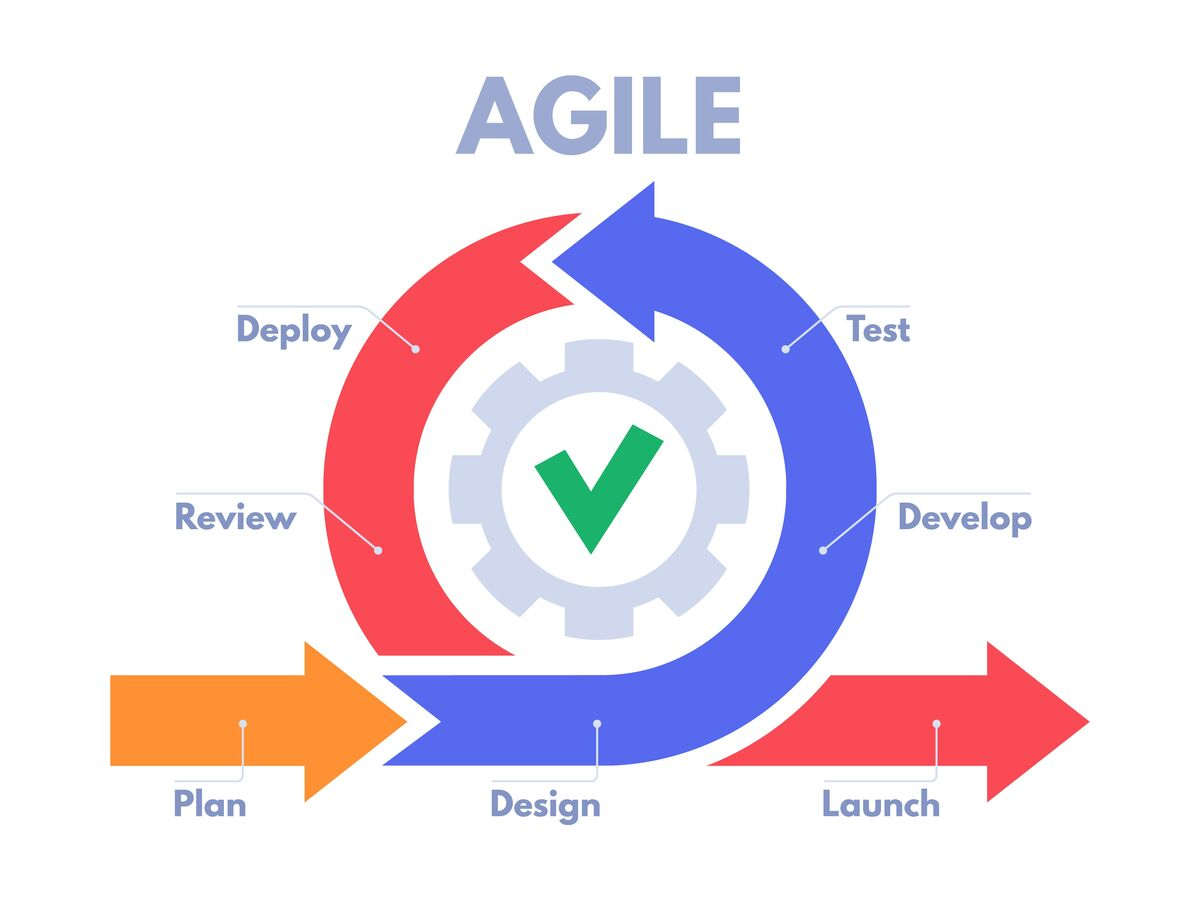
\includegraphics[width=0.7\textwidth]{schema_agile.jpg}
\end{center}

\vspace{0.2cm}

\textbf{Approche :} Développement itératif par sprints de 2 semaines
\end{frame}

\begin{frame}{Phases de Développement}
\begin{columns}
\begin{column}{0.5\textwidth}
\textbf{✅ Phases complétées}
\begin{itemize}
    \item[$\checkmark$] Phase 1 : Infrastructure
    \begin{itemize}
        \item Docker, FastAPI, Next.js
    \end{itemize}
    \item[$\checkmark$] Phase 2 : Streaming vidéo
    \begin{itemize}
        \item HTTP Range, clips
    \end{itemize}
    \item[$\checkmark$] Phase 3 : Recherche ES
    \begin{itemize}
        \item Indexation, full-text
    \end{itemize}
\end{itemize}
\end{column}

\begin{column}{0.5\textwidth}
\begin{itemize}
    \item[$\checkmark$] Phase 4 : Sémantique
    \begin{itemize}
        \item Embeddings, highlights
    \end{itemize}
    \item[$\checkmark$] Phase 5 : Chatbot IA
    \begin{itemize}
        \item RAG, OpenAI
    \end{itemize}
    \item[$\checkmark$] Phase 6 : Tests
    \begin{itemize}
        \item Unitaires, E2E
    \end{itemize}
\end{itemize}

\vspace{0.3cm}

\textbf{Durée :} 12 semaines
\end{column}
\end{columns}
\end{frame}

%=============================================================================
\section{Métriques et Performance}
%=============================================================================

\begin{frame}{Métriques Techniques}
\begin{table}
\centering
\begin{tabular}{|l|c|}
\hline
\textbf{Métrique} & \textbf{Valeur} \\
\hline
Temps réponse API (moyenne) & \textless 100ms \\
Temps recherche ES & \textless 50ms \\
Taille chunks vidéo & 1 MB \\
Dimensions embeddings & 384 \\
Points indexés (2 matchs) & 170 \\
Modalités supportées & 3 (texte, méta, sémantique) \\
Lignes code backend & \textasciitilde4000 \\
Lignes code frontend & \textasciitilde2500 \\
Tests automatisés & 40+ \\
\hline
\end{tabular}
\end{table}

\vspace{0.2cm}

\begin{block}{Performance}
\begin{itemize}
    \item Recherche vectorielle k-NN : 20 résultats en \textless 100ms
    \item Génération embedding : \textasciitilde50ms par point
    \item Streaming vidéo : Seek instantané grâce aux Range Requests
\end{itemize}
\end{block}
\end{frame}

%=============================================================================
\section{Démonstration}
%=============================================================================

\begin{frame}{Démonstration Live}
\begin{enumerate}
    \item \textbf{Navigation} : Galerie de vidéos
    \vspace{0.2cm}
    
    \item \textbf{Lecture} : Lecteur vidéo + navigation clips
    \vspace{0.2cm}
    
    \item \textbf{Recherche textuelle} : 
    \begin{itemize}
        \item Requête : "topspin gagnant set 3"
        \item Filtres : set, gagnant, serveur
    \end{itemize}
    \vspace{0.2cm}
    
    \item \textbf{Mode Highlights} : 
    \begin{itemize}
        \item Détection auto des meilleurs points
        \item Tri par similarité vectorielle
    \end{itemize}
    \vspace{0.2cm}
    
    \item \textbf{Chatbot IA} :
    \begin{itemize}
        \item "Montre-moi les meilleurs échanges longs de Fan Zhendong"
        \item Réponse naturelle + clips suggérés
    \end{itemize}
    \vspace{0.2cm}
    
    \item \textbf{Recommandations} : Points similaires (k-NN)
\end{enumerate}
\end{frame}

%=============================================================================
\section{Prochaines Étapes}
%=============================================================================

\begin{frame}{Roadmap Futur}
\begin{block}{Court terme}
\begin{itemize}
    \item Déploiement sur serveur de production
    \item Indexation de 100+ matchs
    \item Optimisation performances (cache, CDN)
\end{itemize}
\end{block}

\begin{block}{Moyen terme}
\begin{itemize}
    \item \textbf{Analyse audio} : Détection automatique applaudissements
    \item \textbf{Interface admin} : Upload et annotation de matchs
    \item \textbf{Export statistiques} : Rapports PDF, graphiques
\end{itemize}
\end{block}

\begin{block}{Long terme - Scalabilité}
\begin{itemize}
    \item Clustering Elasticsearch (millions de points)
    \item \textbf{Computer Vision} : Détection automatique des coups
    \item Support multi-sports (badminton, squash, etc.)
\end{itemize}
\end{block}
\end{frame}

%=============================================================================
\section{Conclusion}
%=============================================================================

\begin{frame}{Bilan du Projet}
\begin{block}{Objectifs atteints ✅}
\begin{itemize}
    \item[$\checkmark$] Moteur de recherche multimodal fonctionnel
    \item[$\checkmark$] Interface utilisateur intuitive et rapide
    \item[$\checkmark$] Recherche sémantique avec embeddings
    \item[$\checkmark$] Chatbot IA (RAG) avec OpenAI
    \item[$\checkmark$] Architecture scalable et testée
\end{itemize}
\end{block}

\vspace{0.3cm}

\begin{block}{Compétences développées}
\begin{itemize}
    \item Développement Full-Stack moderne (FastAPI + Next.js)
    \item Moteurs de recherche avancés (ES + embeddings vectoriels)
    \item Intelligence Artificielle (RAG, sentence-transformers, OpenAI)
    \item Streaming vidéo optimisé (HTTP Range Requests)
    \item DevOps (Docker, tests automatisés, CI/CD)
\end{itemize}
\end{block}
\end{frame}

\begin{frame}{Impact et Perspectives}
\begin{center}
\Large{\textbf{Démocratisation de l'analyse sportive\\professionnelle vers le grand public}}
\end{center}

\vspace{0.5cm}

\begin{block}{Innovation technique}
\begin{itemize}
    \item Combinaison recherche textuelle + vectorielle + IA générative
    \item Pipeline RAG complet et fonctionnel
    \item Tests E2E pour garantir la qualité
\end{itemize}
\end{block}

\vspace{0.3cm}

\begin{center}
\textbf{Technologies maîtrisées :}\\
Python • TypeScript • React • FastAPI • Elasticsearch\\
Sentence-Transformers • OpenAI • Docker • Playwright
\end{center}
\end{frame}

\begin{frame}{Questions / Réponses}
\begin{center}

\vspace{1cm}

\Large{Questions / Réponses}

\vspace{1cm}

\end{center}

\begin{block}{Ressources}
\begin{itemize}
    \item Code source : GitHub
    \item Documentation : README.md + TESTING.md
    \item Démo live : http://localhost:3000
    \item API Docs : http://localhost:8000/docs
\end{itemize}
\end{block}
\end{frame}

\begin{frame}
\begin{center}
\Huge{Merci pour votre attention !}

\vspace{1cm}

\Large{Questions ?}

\vspace{1cm}

\normalsize
\textbf{Contact :} Projet Informatique\\
\textbf{Stack :} FastAPI • Next.js • Elasticsearch • OpenAI\\
\textbf{GitHub :} Disponible sur demande
\end{center}
\end{frame}

\end{document}
